\documentclass[a4paper]{article}

%% Language and font encodings
\usepackage[english]{babel}
\usepackage[utf8x]{inputenc}
\usepackage[T1]{fontenc}

%% Sets page size and margins
\usepackage[a4paper,top=3cm,bottom=2cm,left=3cm,right=3cm,marginparwidth=1.75cm]{geometry}

%% Useful packages
\usepackage{amsmath}
\usepackage{amssymb}
\usepackage{enumitem}
\usepackage{graphicx}
\usepackage[colorinlistoftodos]{todonotes}
\usepackage[colorlinks=true, allcolors=blue]{hyperref}

\usepackage{latexsym}
\usepackage{sidecap}

\usepackage{tikz}
\usetikzlibrary{decorations.pathreplacing}

\title{Homework 5\\
	601.482/682 Deep Learning\\
	Spring 2019}

\begin{document}
	\maketitle
	
	\centering{
		\textbf{Due Fri. 03/29 11:59pm.\\
			Please submit a latex generated PDF\\
			to Gradescope with entry code MYRR74}}\\
	
	\begin{enumerate}
		% Problem 1
		\item Computing Network Sizes
		\begin{enumerate}
			\item Given the multi-layer perceptron below in Figure 1, compute the number of free parameters for this model (Note that biases are explicitly disregarded in this case).
			\begin{SCfigure}[][h]
				\centering
				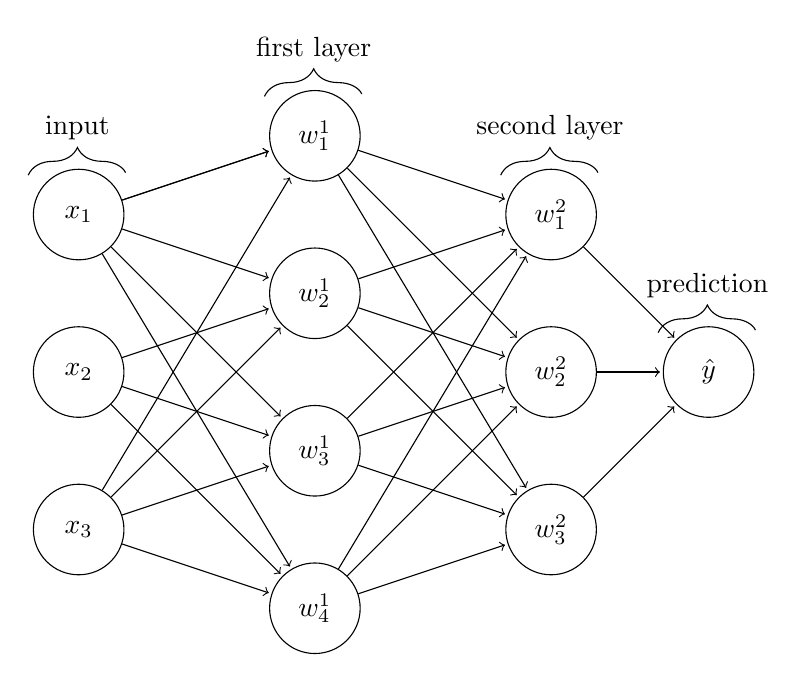
\begin{tikzpicture}[shorten >=1pt]
				\tikzstyle{unit}=[draw,shape=circle,minimum size=1.15cm]
				
				\node[unit](x1) at (0,5){$x_1$};
				\node[unit](x2) at (0,3){$x_2$};
				\node[unit](x3) at (0,1){$x_3$};
				
				\node[unit](w11) at (3,6){$w^1_1$};
				\node[unit](w12) at (3,4){$w^1_2$};
				\node[unit](w13) at (3,2){$w^1_3$};
				\node[unit](w14) at (3,0){$w^1_4$};
				
				\node[unit](w21) at (6,5){$w^2_1$};
				\node[unit](w22) at (6,3){$w^2_2$};
				\node[unit](w23) at (6,1){$w^2_3$};
				
				\node[unit](y) at (8,3){$\hat{y}$};
				
				
				
				\draw[->] (x1) -- (w11);
				\draw[->] (x1) -- (w12);
				\draw[->] (x1) -- (w13);
				\draw[->] (x1) -- (w14);
				
				\draw[->] (x1) -- (w11);
				\draw[->] (x2) -- (w12);
				\draw[->] (x2) -- (w13);
				\draw[->] (x2) -- (w14);
				
				\draw[->] (x3) -- (w11);
				\draw[->] (x3) -- (w12);
				\draw[->] (x3) -- (w13);
				\draw[->] (x3) -- (w14);
				
				
				\draw[->] (w11) -- (w21);
				\draw[->] (w11) -- (w22);
				\draw[->] (w11) -- (w23);
				
				\draw[->] (w12) -- (w21);
				\draw[->] (w12) -- (w22);
				\draw[->] (w12) -- (w23);
				
				\draw[->] (w13) -- (w21);
				\draw[->] (w13) -- (w22);
				\draw[->] (w13) -- (w23);
				
				\draw[->] (w14) -- (w21);
				\draw[->] (w14) -- (w22);
				\draw[->] (w14) -- (w23);
				
				\draw[->] (w21) -- (y);
				\draw[->] (w22) -- (y);
				\draw[->] (w23) -- (y);
				
				\draw [decorate,decoration={brace,amplitude=10pt},xshift=-4pt,yshift=0pt] (-0.5,5.5) -- (0.75,5.5) node [black,midway,yshift=+0.6cm]{input};
				\draw [decorate,decoration={brace,amplitude=10pt},xshift=-4pt,yshift=0pt] (2.5,6.5) -- (3.75,6.5) node [black,midway,yshift=+0.6cm]{first layer};
				\draw [decorate,decoration={brace,amplitude=10pt},xshift=-4pt,yshift=0pt] (5.5,5.5) -- (6.75,5.5) node [black,midway,yshift=+0.6cm]{second layer};
				
				\draw [decorate,decoration={brace,amplitude=10pt},xshift=-4pt,yshift=0pt] (7.5,3.5) -- (8.75,3.5) node [black,midway,yshift=+0.6cm]{prediction};
				\end{tikzpicture}
				\caption{Multi-layer Perceptron}
				\label{fig:perceptron}
			\end{SCfigure}
			\end{enumerate}
			
			In this part, you will analyze the size of a state-of-the-art architecture not discussed in class. In the \href{http://www.image-net.org/challenges/LSVRC/2014/results}{ImageNet ILSVRC 2014} contest, two fairly deep networks performed very well: The \href{https://arxiv.org/pdf/1409.1556.pdf}{VGG} network and the \href{https://www.cs.unc.edu/~wliu/papers/GoogLeNet.pdf}{GoogLeNet}. While VGG performed best in the localization task and ranked second in classification, GoogLeNet won the classification task achieving a top-5 error rate of 6.67\%. Figure \ref{fig:googlenet} presents the architecture of GoogLeNet, which is built up of 9 stacked "inception" modules displayed in Figure \ref{fig:inception}.
		
		\begin{enumerate}[resume]
			\item Consider the layer "inception (3a)" from Table 1(Figure \ref{fig:table} ) in the \href{https://www.cs.unc.edu/~wliu/papers/GoogLeNet.pdf}{GoogLeNet paper}. Notice how "3x3 reduce" and "5x5 reduce" are used between layers - from section 5, this "stands for the number of 1x1 filters in the reduction layer used before the 3×3 and 5×5 convolutions". Compute the number of free parameters for the "inception (3a)" layer.
			
			\item Now, consider that the reduction portion of "3x3 reduce" and "5x5 reduce" were omitted (i.e. no 1x1 filters were used before the 3x3 and 5x5 convolutions). Compute the number of free parameters for this updated "inception (3a)" layer. How does this compare to the original layer?
		\end{enumerate}
		
		\begin{figure}[h]
				\centering
				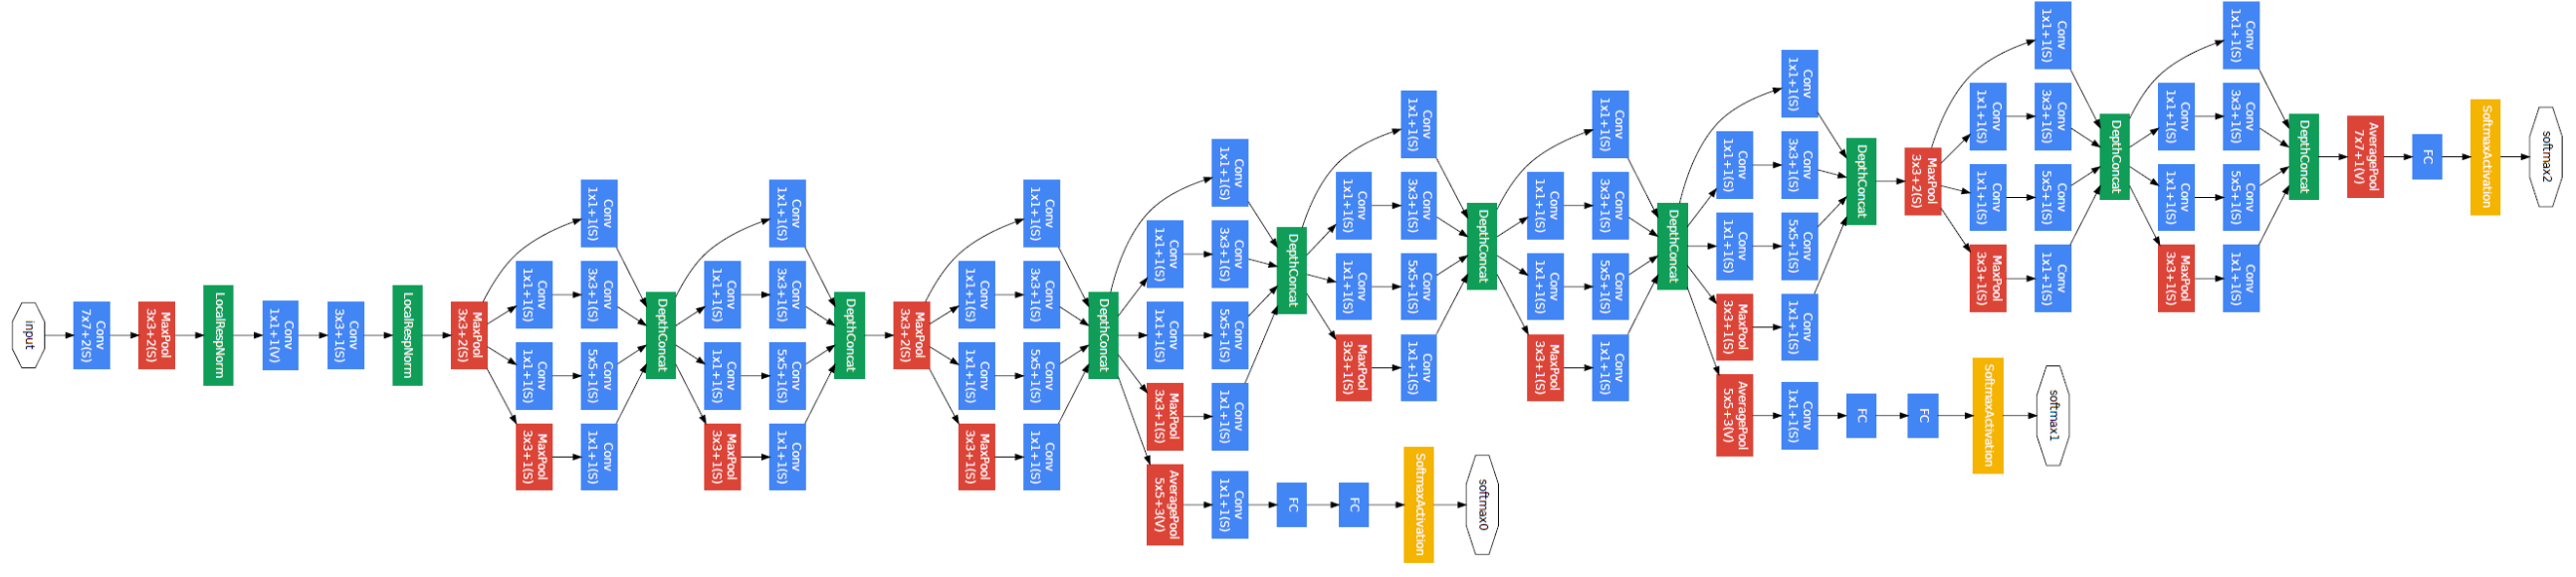
\includegraphics[scale=0.15]{images/googlenet.png}
				\caption{GoogleNet Architecture}
				\label{fig:googlenet}
			\end{figure}
			
			\begin{figure}[h]
				\centering
				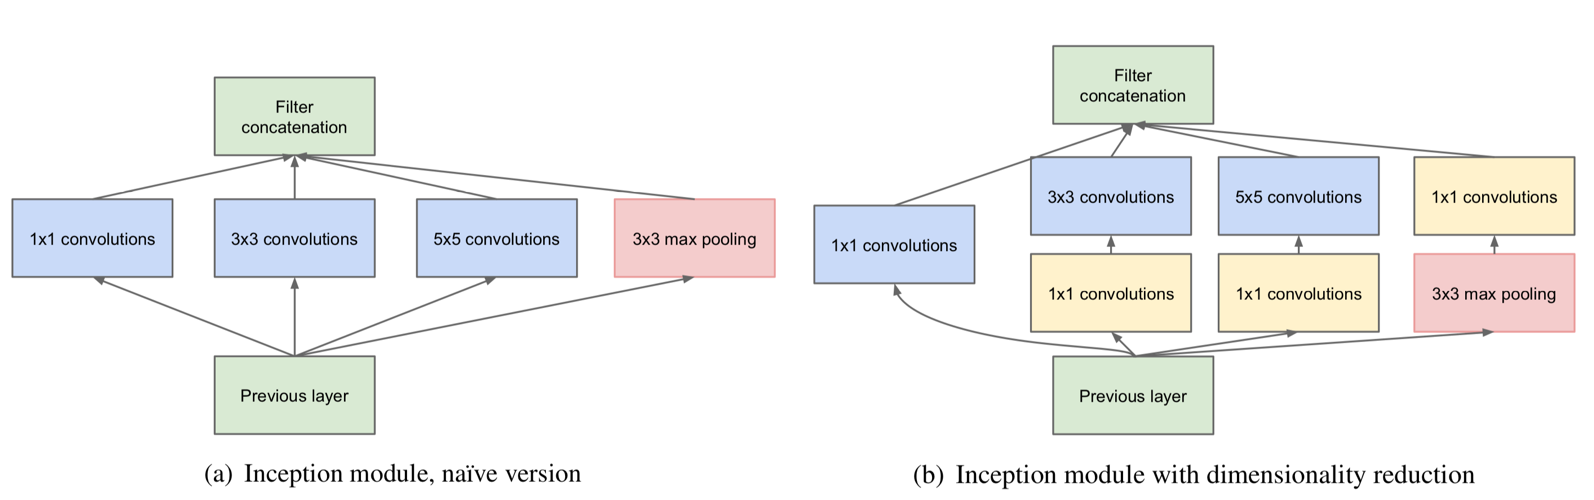
\includegraphics[scale=0.30]{images/inception.png}
				\caption{Inception Module}
				\label{fig:inception}
			\end{figure}
			
			\begin{figure}[!]
				\centering
				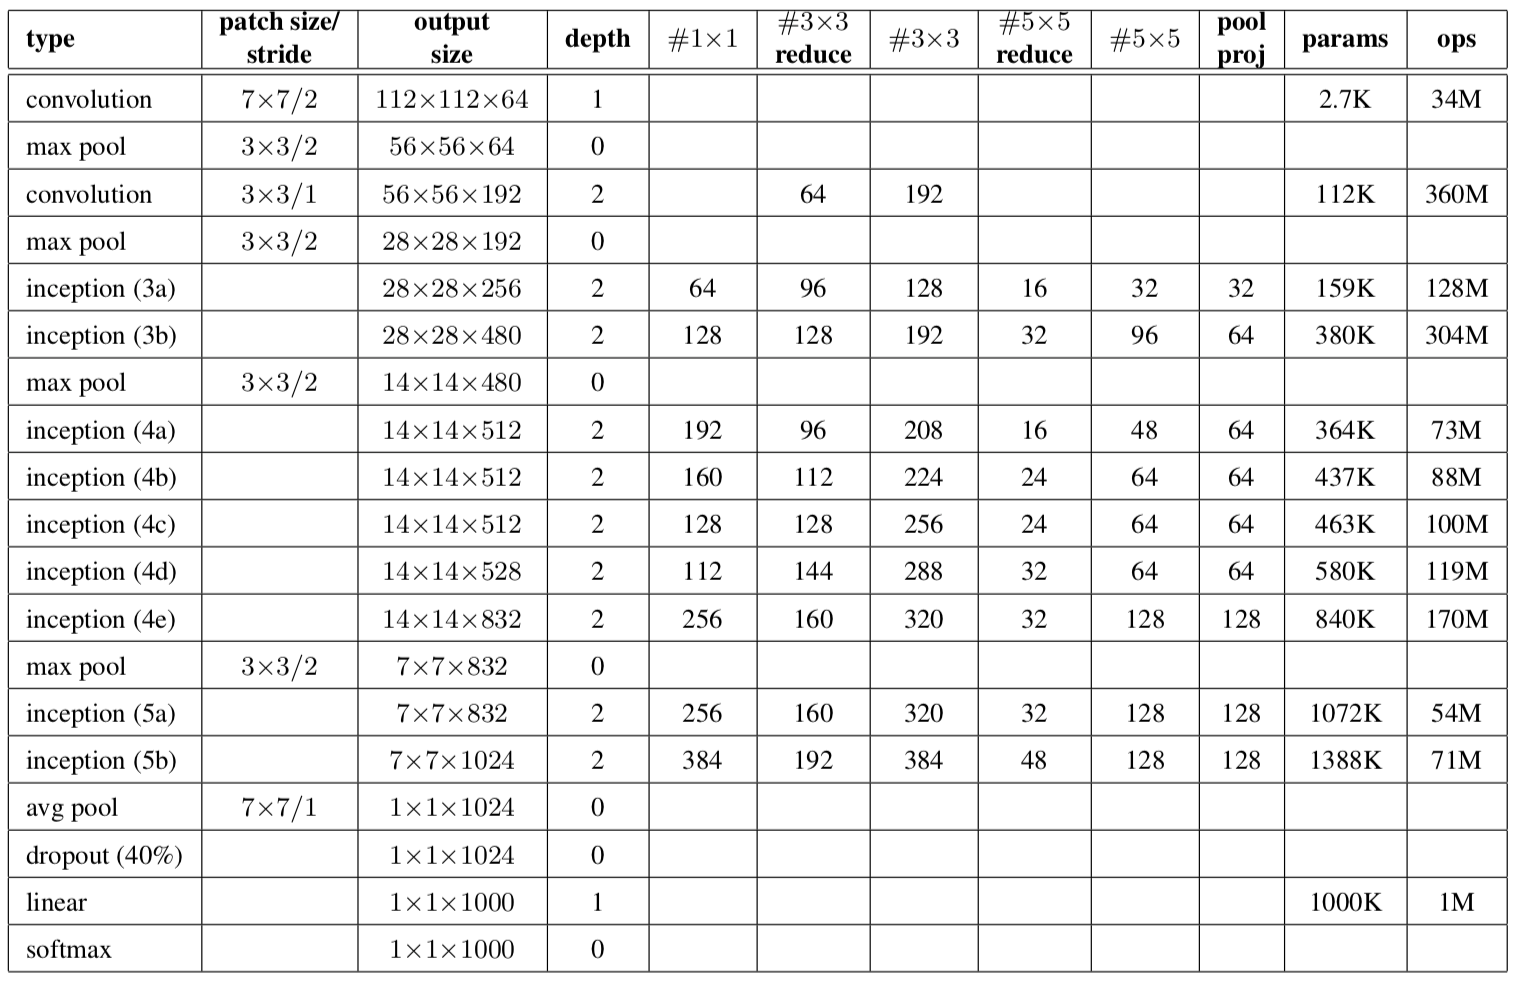
\includegraphics[scale=0.25]{images/table.png}
				\caption{Table 1: GoogLeNet incarnation of the Inception architecture.}
				\label{fig:table}
			\end{figure}
		
		
		\newpage
		\item Receptive Fields
		\begin{enumerate}
			\item Consider the network in Figure \ref{fig:conv}, which is constructed by 2 $5\times5$ convolution kernels. What is the receptive field of one pixel in layer 2? Please draw a 2D graph (excluding the channel dimension) to illustrate your calculation.
			
			\item Now consider that we add a n-by-n max-pooling layer following layer 2. What will be the receptive field after the max-pooling layer?
			
			\begin{figure}[h]
				\centering
				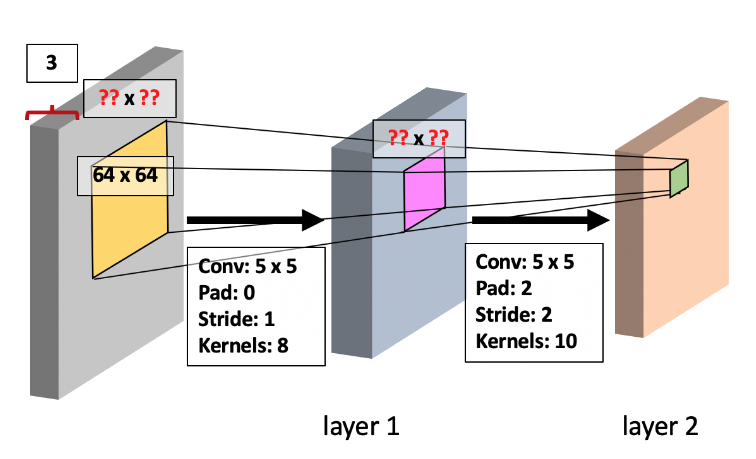
\includegraphics[scale=0.25]{images/conv.png}
				\caption{Convolutional Architecture}
				\label{fig:conv}
			\end{figure}
			
		\end{enumerate}
		
		\newpage
		\item Gradient Descent Optimization
		\begin{enumerate}
			\item Consider Figure \ref{fig:graph}, which depicts a cost function $L(x): \mathbb{R}^2 \rightarrow \mathbb{R}$. The red dot represents the current estimate of $\mathbf{x}_t = [x_1, x_2]$ at time $t$. Please give a rough sketch of the direction of update steps that would be taken by vanilla SGD.
			
			\begin{figure}[h]
				\centering
				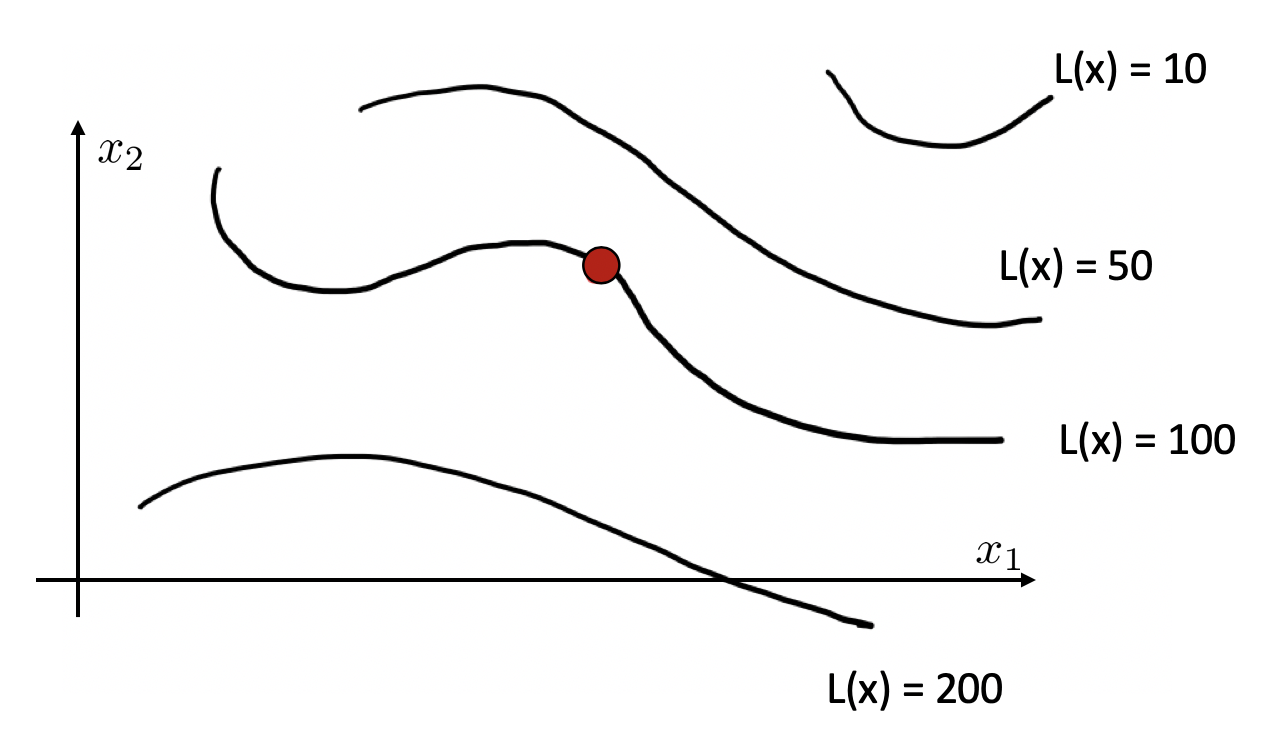
\includegraphics[scale=0.30]{images/graph.png}
				\caption{Contour lines of an arbitrary cost function with current estimate $\mathbf{x}_t$.}
				\label{fig:graph}
			\end{figure}
			
			\item It is worth mentioning that the contour lines shown in Fig.~\ref{fig:graph} will change during optimization since the loss is evaluated over a single batch rather than the whole dataset. As discussed in class, this observation suggests that for unfortunate updates we might get stuck in saddle points, where the vanilla SGD gradient is 0. One way to combat this problem is to use first and/or second order momentum. Please \underline{briefly} explain why these moments are helpful and how they would change the update direction sketched in (a).
			
		\end{enumerate}
	\end{enumerate}
	
\end{document}















